\documentclass[border=4pt]{standalone}
\usepackage{tikz}
\usepackage{amsmath}
\usetikzlibrary{arrows.meta,calc}

\begin{document}
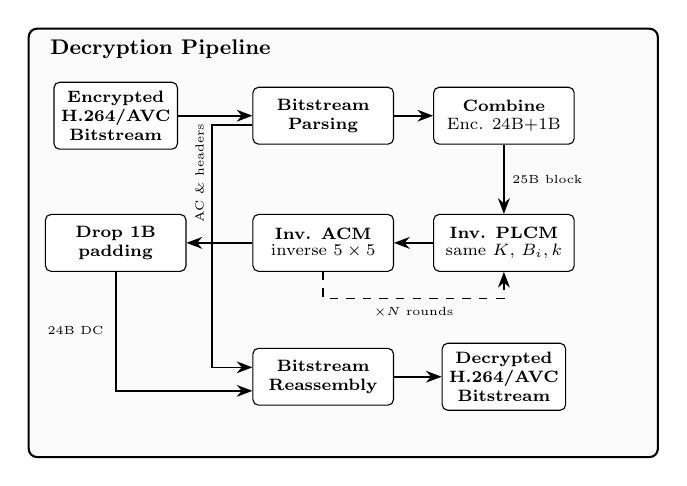
\begin{tikzpicture}[
    scale=0.85, transform shape, % Phù hợp cấu trúc 1 cột báo Q1
    >=Stealth,
    font=\scriptsize,
    arr/.style={->, line width=0.6pt},
    darr/.style={->, dashed, line width=0.6pt},
    frame/.style={draw, rounded corners=3pt, line width=0.75pt, fill=gray!3},
    box/.style={draw, rounded corners=2pt, fill=white, align=center, inner sep=3pt, minimum height=0.85cm},
    sbox/.style={box, minimum width=1.8cm},
    mbox/.style={box, minimum width=2.1cm},
    note/.style={font=\tiny, align=center}
]

% =========================================================
% KHUNG ĐA TIẾN TRÌNH (DECRYPTION PIPELINE)
% =========================================================
\draw[frame] (0,0) rectangle (9.40,-6.40);
\node[anchor=west, font=\bfseries\small] at (0.2,-0.3) {Decryption Pipeline};

% ------------------- HÀNG 1 -------------------
\node[sbox, minimum height=1.0cm] (in) at (1.3,-1.3)
{\textbf{Encrypted}\\\textbf{H.264/AVC}\\\textbf{Bitstream}};

\node[mbox] (parse) at (4.4,-1.3)
{\textbf{Bitstream}\\\textbf{Parsing}};

\node[mbox] (comb) at (7.1,-1.3)
{\textbf{Combine}\\Enc. 24B+1B};

\draw[arr] (in.east) -- (parse.west);
\draw[arr] (parse.east) -- (comb.west);

% ------------------- HÀNG 2 -------------------
\node[mbox] (iplcm) at (7.1,-3.2)
{\textbf{Inv. PLCM}\\[-1pt]
same $K$, $B_i,k$};

\node[mbox] (iacm) at (4.4,-3.2)
{\textbf{Inv. ACM}\\[-1pt]
inverse $5\times5$};

\node[mbox] (drop) at (1.3,-3.2)
{\textbf{Drop 1B}\\\textbf{padding}};

\draw[arr] (comb.south) -- node[right, note, pos=0.5] {25B block} (iplcm.north);
\draw[arr] (iplcm.west) -- (iacm.east);
\draw[arr] (iacm.west) -- (drop.east);

% Vòng lặp phản hồi (Feedback Loop) xN rounds dưới đáy
\draw[darr] (iacm.south) -- ++(0,-0.4) -- node[below, note] {$\times N$ rounds} ($(iplcm.south)+(0,-0.4)$) -- (iplcm.south);

% ------------------- HÀNG 3 -------------------
\node[mbox] (reasm) at (4.4,-5.2)
{\textbf{Bitstream}\\\textbf{Reassembly}};

\node[sbox, minimum height=1.0cm] (out) at (7.1,-5.2)
{\textbf{Decrypted}\\\textbf{H.264/AVC}\\\textbf{Bitstream}};

\draw[arr] (reasm.east) -- (out.west);

% Đường nối từ Drop 1B xuống Reassembly (24B DC) vuông góc 90 độ hoàn chỉnh
\draw[arr] (drop.south) |- node[pos=0.3, above, note, xshift=-0.6cm] {24B DC} ([yshift=-6pt]reasm.west);

% ------------------- ĐƯỜNG BYPASS XUYÊN KHE GIỮA RỘNG (Đã sửa lỗi) -------------------
% Sử dụng dịch điểm tương đối ++(-0.6,0) để lùi vào khe hở X=2.75 mà không bị lỗi cú pháp TikZ
% Góc bẻ bên dưới được đảm bảo vuông góc 90 độ hoàn hảo nhờ toán tử |- 
\draw[arr] ([yshift=-4pt]parse.west) -- ++(-0.6,0) -- 
    node[pos=0.25, left, note, rotate=90, anchor=south] {AC \& headers} 
    ($(parse.west)+(-0.6,-3.0)$) |- ([yshift=4pt]reasm.west);

\end{tikzpicture}
\end{document}